\documentclass[output=paper]{LSP/langsci} 
\ChapterDOI{10.5281/zenodo.1291926}

\title{The META-NET strategic research agenda for language technology   in Europe: {A}n extended summary}
\shorttitlerunninghead{The META-NET Strategic Research Agenda}

\author{Georg Rehm \affiliation{DFKI GmbH}}
 

\abstract{Recognising Europe's exceptional demand and opportunities for  multilingual language technologies, 60 leading research centres in  34 European countries joined forces in \textsc{meta-net}, a European Network   of Excellence. \textsc{meta-net} has developed a Strategic Research Agenda   (\textsc{sra}) for multilingual Europe -- the complex planning and discussion  process took more than two years to complete. While the complete \textsc{sra}  has been published elsewhere \citep{SRA2013}, this heavily condensed  version provides an extended summary as an alternative mode of  access and to enable interested parties to familiarise themselves  with its key concepts in an efficient way.}
 
\maketitle

\begin{document}
  
\section{Introduction}
\label{sec:introduction}

The multilingual setup of our European society imposes grand societal
challenges on political, economic and social integration and
inclusion, especially in the creation of the single digital market and
unified information space targeted by the Digital Agenda
\citep{DA2010}. As many as 21 European languages are at risk of
digital extinction \citep{LWP2012}. They could become victims of the
digital age as they are under-represented online and under-resourced
with respect to language technologies. Huge market opportunities
remain untapped because of language barriers. If no action is taken,
many European citizens will find that speaking their mother tongue
leaves them at a social and economic disadvantage.

Language technology is the missing piece of the puzzle that will bring
us closer to a single digital market. It is the key enabler and
solution to boosting future growth in Europe and strengthening our
competitiveness. The key question is: Will Europe wholeheartedly
decide to participate in this fast growing market?

Although we use computers to write, phones to chat and the web to
search for knowledge, Information Technology (\textsc{it}) does not yet have access to the meaning,
purpose and sentiment behind our trillions of written and spoken
words. Technology will bridge the rift separating \textsc{it} and the human
mind using sophisticated technologies for language
understanding. Today's computers cannot understand texts and questions
well enough to provide translations, summaries or reliable answers,
but in less than ten years such services will be offered for many
languages. Technological mastery of human language will enable a host
of innovative \textsc{it} products and services in commerce, administration,
government, education, health care, entertainment, tourism and other
sectors.

Recognising Europe's exceptional demand and opportunities, 60 leading
research centres in 34 European countries joined forces in \textsc{meta-net}
(\url{http://www.meta-net.eu}), a European Network of Excellence
dedicated to the technological foundations of a multilingual,
inclusive, innovative and reflective European society and partially
supported through several projects funded by the European Commission
(\textsc{ec}). \textsc{meta-net} assembled the Multilingual Europe Technology Alliance
(\textsc{meta}) with more than 700 organisations and experts representing
multiple stakeholders. In addition, \textsc{meta-net} signed collaboration
agreements and memoranda of understanding
\citep[see][]{metanetcolab2013} with more than 40 other projects and
initiatives in the field such as \textsc{clarin} (Common Language Resources and
Technology Infrastructure, \url{http://www.clarin.eu}) and FLaReNet
(Fostering Language Resources Network, \url{http://www.flarenet.eu}).

Working together with numerous organisations and experts from a
variety of fields, \textsc{meta-net} has developed a Strategic Research Agenda
\citep[SRA,][]{SRA2013}. Our recommendations for Multilingual Europe
2020, as specified in the \textsc{sra}, are based on a thorough planning
process involving more than one thousand experts.

We predict, in line with many other forecasts, that the next
generation of \textsc{it} will be able to handle human language, knowledge and
emotion in competent and meaningful ways. These new competencies will
enable an endless stream of novel services that will improve
communication and understanding. Many services will help people learn
about and understand things such as world history, technology, nature
and the economy. Others will help us to better understand each other
across language and knowledge boundaries. They will also drive many
other services including programmes for commerce, localisation, and
personal assistance.

Our ultimate goal is monolingual, crosslingual and multilingual
technology support for all languages spoken by a significant
population in Europe. To achieve this, we recommend focusing on three
priority research topics connected to innovative application scenarios
that will provide European research and development (\textsc{r}\&\textsc{d}) in this field with the ability to
compete with other markets and subsequently achieve benefits for
European society and citizens as well as an array of opportunities for
our economy and future growth. We are confident that upcoming \textsc{eu}
funding programmes, specifically Horizon 2020 \citep{H2020} and
Connecting Europe Facility \citep{CEF2011}, combined with national and
regional funding, can provide the necessary resources for
accomplishing our joint vision.

A recent policy brief \citep{bruegel12} proposes that Europe
specialises in new \textsc{ict} (Information and Communications Technology)
sectors as a means for post-crisis recovery. The European problem lies
less in the generation of new ideas than in their successful
commercialisation. The study identifies major obstacles: the lack of a
single digital market, and the absence of \textsc{ict} clusters and powerful
platform providers. It suggests that the \textsc{eu} policy framework could
overcome these barriers and leverage the growth potential of new \textsc{ict}
markets by extending research and infrastructure funding to
pre-commercial projects, in particular those involving the creation of
\textsc{ict} clusters and platforms. This is exactly the goal we are trying to
achieve. Our recommendations envisage five lines of action for
large-scale research and innovation. First, there are three priority
research themes: \emph{Translingual Cloud}, \emph{Social Intelligence
  and e-Participation} and \emph{Socially Aware Interactive
  Assistants}. The other two themes focus upon \emph{Core Technologies
  and Resources for Europe's Languages} and a \emph{European Service
  platform for Language technologies}.

The objective of the priority research themes is to turn our joint
vision into reality and allow Europe to benefit from a technological
revolution that will overcome barriers of understanding between people
of different languages, people and technology, and people and the
digitised knowledge of mankind.

\section{Multilingual Europe: Facts and opportunities}
\label{sec:background-context}

During the last 60 years, Europe has become a distinct political and
economic structure. Culturally and linguistically it is rich and
diverse. However, everyday communication between Europe's citizens,
enterprises and politicians is inevitably confronted with language
barriers. They are an invisible and increasingly problematic threat to
economic growth \citep{economist12}. The \textsc{eu}'s institutions spend about
\emph{one billion Euros per year} on translation and interpretation to
maintain their policy of multilingualism \citep{EC7} and the overall
European market for translation, interpretation, software localisation
and website globalisation was estimated at 5.7 billion Euros in 2008.

The only -- unacceptable and rather un-European -- alternative to a
multilingual Europe would be to allow a single language to take a
predominant position and replace all other languages in transnational
communication. Another way to overcome language barriers is to learn
foreign languages. Given the 23 official \textsc{eu} languages plus 60 or more
other languages spoken in Europe \citep{eurobarometer2012}, language
learning alone cannot solve the problem. Without technological
support, our linguistic diversity will be an insurmountable obstacle
for the entire continent. Only about half of the 500 million people
who live in the \textsc{eu} speak English. There is no such thing as a lingua
franca shared by the vast majority of the population.

Less than 10\% of the \textsc{eu}'s population are willing or able to use
online services in English, which is why multilingual technologies are
badly needed to support and to move the \textsc{eu} online market from more
than 20 language-specific sub-markets to one unified single digital
market with more than 500 million users and consumers. The current
situation with ``many fragmented markets'' is considered one of the
main obstacles that seriously undermine Europe's efforts to exploit
\textsc{ict} fully \citep{DA2010}.

Language technology is a key enabler for sustainable, cost-effective
and socially beneficial solutions to overcome language barriers. It
will offer European stakeholders tremendous advantages, not only
within the European market, but also in trade relations with
non-European countries, especially emerging economies.

In the late 1970s the \textsc{eu} realised the relevance of language technology
as a driver of European unity and began funding its first research
projects, such as \textsc{eurotra}. After a longer period of sparse funding
\citep{euromap, laz1}, the European Commission set up a department
dedicated to language technology and machine translation a few years
ago. Selective funding efforts have led to a number of valuable
results. For example, the \textsc{ec}'s translation services now use Moses,
which has been mainly developed in European research
projects. However, these never led to a concerted European effort
through which the \textsc{eu} and its member states systematically pursue the
common goal of providing technology support for all European
languages.

Europe now has a well-developed research base. Through initiatives
such as \textsc{clarin} and \textsc{meta-net} the community is well connected and
engaged in a long term agenda that aims gradually to strengthen
language technology's role. What is missing in Europe is awareness,
political determination and political will that would take us to a
leading position in this technology area through a concerted funding
effort. This major dedicated push needs to include the political
determination to modify and to adopt a shared, \textsc{eu}-wide language policy
that foresees an important role for language technologies.

Europe's more than 80 languages are one of its richest and most
important cultural assets, and a vital part of its unique social model
\citep{EC2,eurobarometer2012}. While languages such as English and
Spanish are likely to thrive in the emerging digital marketplace, many
European languages could become marginal in a networked society. This
would weaken Europe's global standing and run counter to the goal of
ensuring equal participation for every European citizen regardless of
language. A recent \textsc{unesco} report on multilingualism states that
languages are an essential medium for the enjoyment of fundamental
rights, such as political expression, education and participation in
society \citep{Unesco1,ifa2008,ifa2011,maaya2012}.

Many Europeans find it difficult to interact with online services and
participate in the digital economy. According to a recent study, only
57\% of internet users in Europe purchase goods and services in
languages that are not their native language. Fifty-five percent of users read
content in a foreign language while only 35\% use another language to
write e-mails or post comments on the web \citep{EC1}. A few years
ago, English might have been the lingua franca of the web but the
situation has now drastically changed. The amount of online content in
other European as well as Asian and Middle Eastern languages has
exploded \citep{Ford11}. Already today, more than 55\% of web-based
content is not in English.

The European market for translation, interpretation and localisation
was estimated to be 5.7 billion Euros in 2008. The subtitling and
dubbing sector was at 633 million Euros, while language teaching at 1.6
billion Euros. The overall value of the European language industry was
estimated at 8.4 billion Euros and expected to grow by 10\% per year,
i.\,e., resulting in ca.~16.5 billion Euros in 2015 \citep{EC3,
  EC6}. Yet, this existing capacity is not enough to satisfy current
and future needs, e.\,g., with regard to translation
\citep{csa2009}. Already today, Google Translate translates the same
volume per day that all human translators on the planet translate in
one year \citep{och12}.

\newpage 
Despite recent improvements, the quality, usability and integration of
machine translation into other online services is far from what is
needed. If we rely on existing technologies, automated translation and
the ability to process a variety of content in a variety of languages
will be impossible. The same applies to information services, document
services, media industries, digital archives and language teaching.
The most compelling solution for ensuring the breadth and depth of
language usage in tomorrow's Europe is to use appropriate
technology. Still, the quality and usability of current technologies
is far from what is needed. Especially the smaller European languages
suffer severely from under-representation in the digital realm.

Drawing on the insights gained so far, today's hybrid language
technology mixing deep processing with statistical methods could be
able to bridge the gap between all European languages and beyond. In
the end, high-quality language technology will be a must for all of
Europe's languages for supporting the political and economic unity
through cultural diversity. The three priority research themes are
mainly aimed at Horizon 2020 \citep{H2020}. The more infrastructural
aspects, platform design and implementation and concrete language
technology services are aimed at \textsc{cef} \citep{CEF2011}. An integral
component of our strategic plans are the member states and associated
countries: it is of utmost importance to set up, under the umbrella of
the \textsc{sra}, a coordinated initiative both on the national (member states,
regions, associated countries) and international level (\textsc{ec/eu}),
including research centres as well as small, medium and large
enterprises who work on or with language technologies.

\section{How can language technology help?}
\label{sec:how-can-language-technology-help}

We believe that \emph{Language Technology made in Europe for Europe}
will significantly contribute to future European cross-border and
cross-language communication, economic growth and social stability
while establishing for Europe a worldwide, leading position in
technology innovation, securing Europe's future as a world-wide trader
and exporter of goods, services and information. There are many
societal changes and challenges as well as economic and technological
trends that confirm the urgent need to include sophisticated language
technology in our European \textsc{ict} infrastructure. Among these changes and
challenges are language barriers \citep{EC4}, an ageing population,
people with disabilities, immigration and integration, personal
information services and customer care, operation and cooperation on a
global scale, preservation of cultural heritage, linguistic diversity
\citep{worldsummit2003,Unesco2}, social media and e-participation as
well as market awareness and customer acceptance. \largerpage %Widow

\newpage
Multilingualism has become the global norm rather than the exception
\citep{maaya2012}. Future applications that embed information and
communication technology require sophisticated language
technologies. Fully speech-enabled autonomous robots could help in
disaster areas by rescuing travellers trapped in vehicles or by giving
first aid. Language technology can significantly contribute towards
improving social inclusion and can help us provide answers to urgent
social challenges while creating genuine business opportunities.
Language technology can now automate the very processes of
translation, content production, and knowledge management for all
European languages. It can also empower intuitive
language/speech-based interfaces for household electronics, machinery,
vehicles, computers and robots.

\section{Language technology 2012: Current state}
\label{sec:LT-2012}

Answering the question on the current state of a whole \textsc{r}\&\textsc{d} field is
both difficult and complex. For language technology, even though
partial answers exist in terms of business figures, scientific
challenges and results from educational studies, nobody has collected
these indicators and provided comparable reports for a substantial
number of European languages yet. In order to arrive at a
comprehensive answer, \textsc{meta-net} prepared the White Paper Series
``Europe's Languages in the Digital Age'' \citep{LWP2012} that
describes the current state of language technology support for 30
European languages (including all 23 official \textsc{eu} languages). This
immense undertaking has been in preparation since mid 2010 and was
published in the Summer of 2012. More than 200 experts participated to
the 30 volumes as co-authors and contributors.

The differences in technology support between the various languages
and areas are dramatic and alarming. In all of the four areas we
examined (machine translation, speech processing, text analytics,
language resources), English is ahead of the other languages but even
support for English is far from being perfect. While there are good
quality software and resources available for a few larger languages
and application areas, others, usually smaller or very small
languages, have substantial gaps. Many languages lack even basic
technologies for text analytics and essential language
resources. Others have basic resources but the implementation of
semantic methods is still far away. Currently no language, not even
English, has the technological support it deserves. Also, the number
of badly supported and under-resourced languages is unacceptable if we
do not want to give up the principles of solidarity and subsidiarity
in Europe.

\newpage 
The \textsc{meta-net} White Paper Series is fully available online at
\url{http://www.meta-net.eu/whitepapers}. On this website we also
present the press release ``At least 21 European Languages in Danger
of Digital Extinction'' which was circulated on the occasion of the
European Day of Languages 2012 (Sept.~26), and also its impact around
the world. The echo generated by our press release shows that Europe
is very passionate and concerned about its languages and that it is
also very interested in the idea of establishing a solid language
technology base for overcoming language barriers.

\section{Language technology 2020: The \textsc{meta-net} technology vision}
\label{sec:lang-techn-2020}

We believe that in the next \textsc{it} revolution computers will master our
languages. Just as they already understand measurements and formats
for dates and times, the operating systems of tomorrow will
\emph{know} human languages. They may not reach the linguistic
performance of educated people and they will not yet know enough about
the world to understand everything, but they will be much more useful
than they are today and will further enhance our work and life.

The broad area of \textsc{communication among people} will see a
dramatically increased use of sophisticated language technology (\textsc{lt}). By the year 2020, with
sufficient research effort on high-quality automatic translation and
robust accurate speech recognition, reliable dialogue translation for
face-to-face conversation and telecommunication will be possible for
at least hundreds of languages, across multiple subject fields and
text types, both spoken and written. Authoring software will check for
appropriate style according to genre and purpose and help evaluate
comprehensibility. It will flag potential errors, suggest corrections,
and use authoring memories to suggest completions of started sentences
or even whole paragraphs. By 2020 tele-meetings will be the norm for
professional meetings. \textsc{lt} will be able to record, transcribe, and
summarise them. Brainstorming will be facilitated by semantic lookup
and structured display of relevant data, proposals, pictures, and
maps. Business email will be embedded in semantic process models to
automate standardised communication. Even before 2020, email
communication will be semantically analysed, checked for sentiment
indicators, and summarised in reports. Semantic integration into work
processes, threading, and response management will be applied across
channels, as will machine translation and analytics.
 
Human language will become the primary medium for
\textsc{communication between people and technology}. The
voice-control interfaces we see today for smart\-phones and search engines are just
the modest start of overcoming the communication barrier between
humankind and the non-human part of the world. Only a few years ago
the idea of talking to a car to access key functions would have seemed
absurd, yet it is now commonplace. Recently the concept of a personal
digital assistant has increased in popularity. We will soon see much
more sophisticated virtual personalities with expressive voices,
faces, and gestures. They will become an interface to any information
provided online. The metaphor of a personal assistant is powerful and
extremely useful, since such an assistant can be made sensitive to the
user's preferences, habits, moods, and goals. By the year 2020 we
could have a highly personalised, socially aware and interactive
virtual assistant. Having been trained on the user's behaviour and
communication space, it will proactively offer advice and it will be
able to speak in the language and dialect of the user but also digest
information in other natural and artificial languages and formats. The
assistant will translate or interpret without the user even needing to
request it. By 2020 there will be a competitive landscape of
intelligent interfaces to all kinds of objects and services employing
human language and other modes for effective communication. 

In the context of the Semantic Web, Linked Open Data and the general
semantification of the web as well as knowledge acquisition and
ontology population, \textsc{lt} can perform many tasks in the
\textsc{processing of knowledge and information}. It can sort,
categorise, catalogue, and filter content and it can deliver the data
for data mining in texts. \textsc{lt} can connect web documents with meaningful
hyperlinks and it can produce summaries of larger text
collections. Opinion mining and sentiment analysis can find out what
people think about products, personalities, or problems and analyse
their feelings about such topics. In the next few years we will see
considerable advances for all these techniques. For large parts of
research and application development, language processing and
knowledge processing will merge. The predicted and planned use of
language and knowledge technologies for social intelligence
applications will involve text and speech analytics, translation,
summarisation, opinion mining, sentiment analysis, and several other
technologies. In 2020, \textsc{lt} will enable forms of knowledge evolution,
transmission and exploitation that speed up scientific, social, and
cultural development. The effects for other knowledge-intensive
application areas such as business intelligence, scientific knowledge
discovery, and multimedia production will be immense.

The wide range of novel or improved applications in our shared vision
represents only a fragment of the countless opportunities for \textsc{lt} to
change our work and everyday life. Language-proficient technology will
enable or enhance applications wherever language is present. It will
change the production, management, and use of patents, legal
contracts, medical reports, recipes, technical descriptions, and
scientific texts, and it will permit many new voice applications such
as automatic services for the submission of complaints and
suggestions, for accepting orders, and for counselling in
customer-care, e-government, education, community services, etc.

\section{Language technology 2020: The \textsc{meta-net} priority research themes}
\label{sec:lang-techn-2020-pts}

In ten years or less, basic language proficiency is going to be an
integral component of any advanced \textsc{it}. It will be available to any
user interface, service and application. Additional language skills
for semantic search, knowledge discovery, human-technology
communication, text analytics, language checking, e-learning,
translation and other applications will employ and extend the basic
proficiency. The shared basic language competence will ensure
consistency and interoperability among services. Many adaptations and
extensions will be derived and improved through sample data and
interaction with people by powerful machine learning techniques.

In the envisaged big push toward realising this vision by massive
research and innovation, the technology community is faced with three
enormous challenges:

\begin{description}
\sloppy
\item[Richness and diversity.] A serious challenge is the sheer
  number of languages, some closely related, others distantly
  apart. Within a language, technology has to deal with dialects,
  sociolects, registers, jargons, genres and slangs.
\item[Depth and meaning.] Understanding language is a complex
  process. Human language is not only the key to knowledge and
  thought, it also cannot be interpreted without shared knowledge and
  active inference. Computational language proficiency needs semantic
  technologies.
\item[Multimodality and grounding.] Human language is embedded
  in our daily activities. It is combined with other modes and media
  of communication. It is affected by beliefs, desires, intentions and
  emotions and it affects all of these. Successful interactive
  language technology requires models of embodied and adaptive human
  interaction with people, technology and other parts of the world.
\end{description}
 
It is fortunate for research and economy that the only way to
effectively tackle the three challenges involves submitting the
evolving technology continuously to the growing demands and practical
stress tests of real world applications. Only a continuous stream of
technological innovation can provide the economic pull forces and the
evolutionary environments for the realisation of the grand vision.

We propose five major action lines of research and innovation:

\begin{itemize}
\sloppy
\item Three Priority Research Themes along with application
  scenarios to drive research and innovation. These will demonstrate
  novel technologies in show-case solutions with high economic and
  societal impact. They will open up numerous new business
  opportunities for European language-technology and -service
  providers.
  \begin{description}
  \item[1.~Translingual Cloud:] generic and specialised federated
    cloud services for instantaneous reliable spoken and written
    translation among all European and major non-European languages.
  \item[2.~Social Intelligence and e-Participation:]
    understanding and dialogue within and across communities of
    citizens, customers, clients and consumers to enable
    e-participation and more effective processes for preparing,
    selecting and evaluating collective decisions.
  \item[3.~Socially Aware Interactive Assistants] that learn and
    adapt and that provide proactive and interactive support tailored
    to specific situations, locations and goals of the user through
    verbal and non-verbal multimodal communication.
  \end{description}
\item The other two themes focus upon base technologies and a service platform:
  \begin{description}
\sloppy
  \item[4.~Core technologies and resources for Europe's
      languages:] a steadily evolving system of shared, collectively
    maintained interoperable core technologies and resources for the
    languages of Europe and selected other languages. These will
    ensure that our languages will be sufficiently supported and
    represented in the next generations of \textsc{it}.
  \item[5.~A European service platform for language
      technologies] for supporting research and innovation by testing
    and showcasing research results, integrating various services,
    even including professional human services, will allow small to medium enterprise (\textsc{sme})  
    providers to offer component and end-user services, and share and
    utilise tools, components and data resources.
  \end{description}
\end{itemize}


These priority themes have been designed with the aim of turning our
vision into reality and to letting Europe benefit from a technological
revolution that will overcome barriers of understanding between people
of different languages, between people and technology and between
people and the knowledge of mankind. The themes connect societal needs
with \textsc{lt} applications.

\subsection{Priority theme 1: Translingual cloud}
\label{sec:priority-theme-1-translation-cloud}

The goal is a multilingual European society, in which all citizens can
use any service, access all knowledge, enjoy all media and control any
technology \emph{in their mother tongues}. This will be a world in
which written and spoken communication is not hindered anymore by
language barriers and in which even specialised high-quality
translation will be affordable. The citizen, the professional, the
organisation, or the software application in need of cross-lingual
communication will use a single access point for channelling text or
speech through a gateway that will instantly return the translations
into the requested languages in the required quality and desired
format. Behind this access point will be a network of generic and
special-purpose services combining automatic translation or
interpretation, language checking, post-editing, as well as human
creativity and quality assurance.

\begin{figure*}[htb]
  \center
  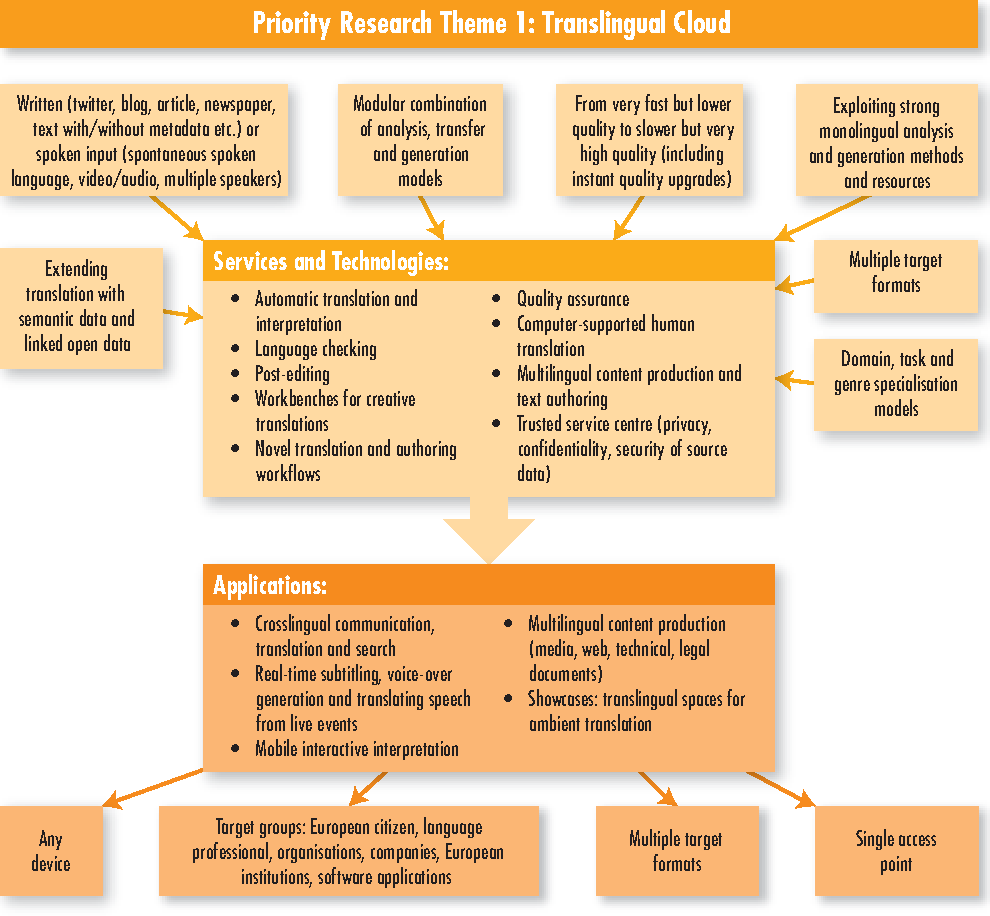
\includegraphics[width=0.7\textwidth]{figures/PT1}
  \caption{Priority Research Theme 1: Translingual Cloud}
  \label{fig:pt1-overview}
\end{figure*}

\newpage %Orphan
One key component of this service (see \figref{fig:pt1-overview})
is a use and provision platform for providers of computer-supported
top-quality human translation, multilingual text authoring and quality
assurance by experts. Other important components are trusted service
centres as certified service providers fulfilling highest standards
for privacy, confidentiality and security of source data and
translations and quality upscale models embedded into services
permitting instant quality upgrades if the results of the requested
service levels do not yet fulfil the quality requirements.


\subsection{Priority theme 2: Social Intelligence and e-Participation}
\label{sec:priority-theme-2-social-intelligence}

The central goal behind the second theme is to use information
technology and the digital content of the web for improving
effectiveness and efficiency of deci\-sion-making in business and
society (see \figref{fig:pt2-overview}). Social intelligence
builds on improved text analytics methodologies but goes far beyond
the analysis. One goal is the analysis of large volumes of social
media, comments, blogs, forum postings etc.~of citizens, customers,
consumers and other stakeholder communities. Part of the analysis is
directed to the status, opinions and acceptance associated with the
individual information units. As the formation of collective opinions
and attitudes is highly dynamic, new developments need to be detected
and trends analysed. As emotions play an important part in individual
actions such as voting, buying, supporting, donating and in collective
opinion formation, the analysis of sentiment is a crucial component of
social intelligence.
 
Social intelligence can also support collective deliberation
processes. Today any collective discussion processes involving large
numbers of participants are bound to become intransparent and
incomprehensible rather fast. By recording, grouping, aggregating and
counting opinion statements, pros and cons, supporting evidence,
sentiments and new questions and issues, the discussion can be
summarised and focussed. Decision processes can be structured,
monitored, documented and visualised, so that joining, following and
benefitting from them becomes much easier. The efficiency and impact
of such processes can thus be greatly enhanced.
 
\begin{figure*}[htb]
  \center
  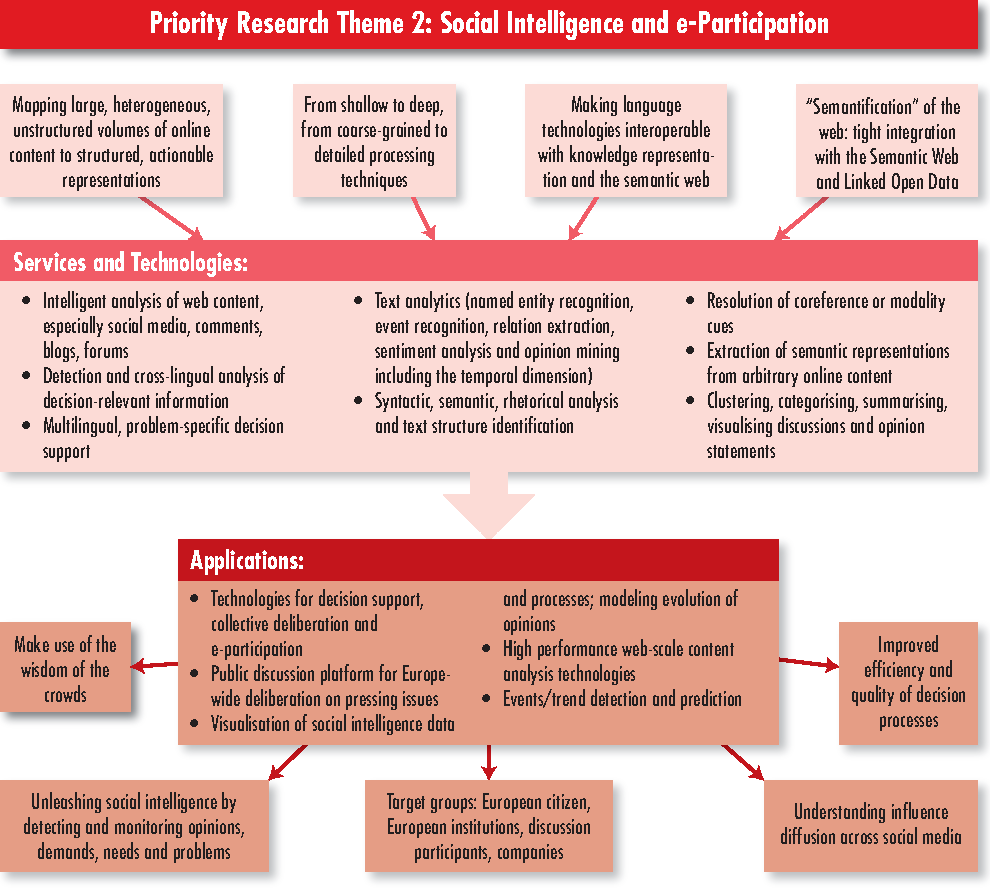
\includegraphics[width=0.7\textwidth]{figures/PT2}
  \caption{Priority Research Theme 2: Social Intelligence and e-Participation}
  \label{fig:pt2-overview}
\end{figure*}

A key enabler will be technologies that can map large, heterogeneous,
and, to a large extent, unstructured volumes of online content to
actionable representations that support decision making and analytics
tasks. Such mappings can range from the relatively shallow to the
relatively deep, encompassing coarse-grained topic classification at
the document or paragraph level or the identification of named
entities, as well as in-depth syntactic, semantic and rhetorical
analysis at the level of individual sentences and beyond or the
resolution of co-reference or modality cues within and across
sentences. Technologies such as, e.\,g., information extraction, data
mining, automatic linking and summarisation have to be made
interoperable with knowledge representation and semantic web
methods. Drawing expertise from related areas such as knowledge
management, information sciences, or social sciences is a prerequisite
to meet the challenge of modelling social intelligence
\citep{ltds2012}.

\subsection{Priority theme 3: Socially aware interactive assistants}
\label{sec:priority-theme-3-interactive-assistant}

Socially aware interactive assistants are conversational agents (see
\figref{fig:pt3-overview}). Their socially-aware behaviour is a
result of combining analysis methods for speech, non-verbal and
semantic signals. They support people interacting with their
environment, including human-computer, human-agent/robot, and
com\-pu\-ter-mediated human-human interaction. The assistants must be able
to act in various environments, both indoor, outdoor and virtual
environments, and also be able to communicate, exchange information
and understand other agents' intentions. They must be able to adapt to
the user's needs and environment and have the capacity to learn
incrementally from all interactions and other sources of information.
\largerpage %Widow

The ideal socially aware multilingual assistant can interact naturally
with humans in any language and modality. It can adapt and be
personalised to individual communication abilities, including special
needs (for the visual, hearing, or motor impaired), affections, or
language proficiencies. It can recognise and generate speech
incrementally and fluently. It is able to assess its performance and
recover from errors. It can learn, personalise itself and forget. It
can assist in language training and education, and provide synthetic
multimedia information analytics.

\begin{figure*}[htb]
  \center
  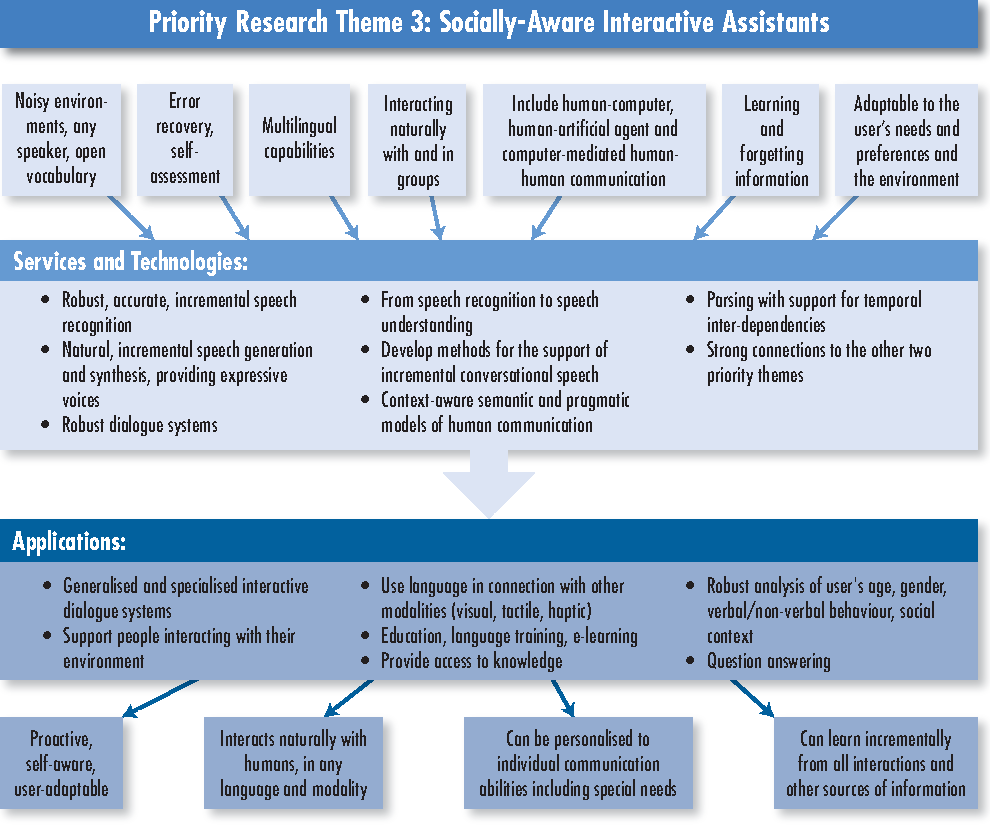
\includegraphics[width=0.7\textwidth]{figures/PT3}
  \caption{Priority Research Theme 3: Socially Aware Interactive Assistants}
  \label{fig:pt3-overview}
\end{figure*}

In addition to significantly improving core speech and language
technologies, the development of socially aware interactive assistants
requires several research breakthroughs. With regard to speech
recognition, accuracy and robustness have to be improved. Methods for
self-assessment, self-adaptation, personalisation, error-recovery,
learning and forgetting information, and also for moving from
recognition to understanding have to be developed. Concerning speech
synthesis, voices have to be made more natural and expressive, control
parameters have to be included for linguistic meaning, speaking style,
emotion, etc. They also have to be equipped with methods for
incremental conversational speech, including filled pauses and
hesitations. 

\subsection{Theme 4: Core language resources and technologies}
\label{sec:sharing-resources-and-results}

The three priority research themes share a large and heterogeneous
group of core technologies for language analysis and production that
provide development support through basic modules and datasets (see
\figref{fig:priority-themes}). To this group belong tools and
technologies such as, among others, tokenisers, part-of-speech
taggers, parsers, tools for building language models, information
retrieval tools, machine learning toolkits, speech recognition and
speech synthesis engines, and integrated architectures. Many of these
tools depend on specific datasets (i.\,e., language resources), for
example, very large collections of linguistically annotated documents
(monolingual or multilingual, aligned corpora), treebanks, grammars,
lexicons, terminologies, dictionaries, ontologies and
language models. Both tools and resources can be rather general or
highly task- or domain-specific, tools can be language-independent,
while datasets are, by definition, language-specific. There are also several
types of resources, such as corpora for machine translation or spoken
dialogue corpora specific to one or more of the priority themes.

A key component of this research agenda is to collect, develop and
make available core technologies and resources through a shared
infrastructure so that the research and technology development carried
out in all themes can make use of them. Over time, this approach will
improve the core technologies, as the specific research will have
certain requirements on the software, extending their feature sets,
performance, accuracy, etc.~through dynamic push-pull
effects. Conceptualising these technologies as a set of shared core
technologies will have positive effects on their sustainability and
interoperability. Also, many European languages other than English are
heavily under-resourced \citep{LWP2012}.

The European academic and industrial technology community is fully
aware of the need for sharing resources such as language data,
language descriptions, tools and core technology components as a basis
for the successful development and implementation of the priority
themes. Initiatives such as FLaReNet \citep{flarenetsra2011} and
\textsc{clarin} have prepared the ground for a culture of sharing, \textsc{meta-net}'s
open resource exchange infrastructure, \textsc{meta-share}, is providing the
technological platform as well as legal and organisational schemes
(see \url{http://www.meta-share.eu}). All language resources and basic
technologies will be created under the core technologies umbrella.

\subsection{Theme 5: A European service platform for language technologies}
\label{sec:europ-service-platform}

We recommend the design and implementation of an ambitious large-scale
platform as a central motor for research and innovation in the next
phase of \textsc{it} evolution and as a ubiquitous resource for the
multilingual European society. The platform will be used for testing,
showcasing, proof-of-concept demonstration, avant-garde adoption,
experimental and operational service composition, and fast and
economical service delivery to enterprises and end-users (see
\figref{fig:platform-overview}). The creation of a cloud platform
for a wide range of services dealing with human language, knowledge
and emotion will not only benefit the individual and corporate users
of these technologies but also the providers. Large-scale \textsc{ict}
infrastructures and innovation clusters such as this one are foreseen
in the Digital Agenda for Europe \citep[24]{DA2010}.

A top layer consists of \textsc{language processing} such as text
filters, tokenisation, spell, grammar and style checking, hyphenation,
lemmatising and parsing. At a deeper level, services will be offered
that realise some degree and form of \textsc{language understanding}
including entity and event extraction, opinion mining and
translation. Both basic language processing and understanding will be
used by services that support \textsc{human communication} or realise
human-machine interaction. Part of this layer are question answering
and dialogue systems as well as email response applications. Another
component will bring in services for processing and storing
\textsc{knowledge} gained by and used for understanding and
communication. This part will include repositories of linked data and
ontologies. These in turn permit a certain range of rational
capabilities often attributed to a notion of intelligence. The goal is
not to model the entire human intelligence but rather to realise
selected forms of \textsc{inference} that are needed for utilising and
extending knowledge, for understanding and for successful
communication. These forms of inference permit better decision
support, pro-active planning and autonomous adaptation. A final part
of services will be dedicated to \textsc{human emotion}. Since people
are largely guided by their emotions and strongly affected by the
emotions of others, truly user-centred \textsc{it} need facilities for
detecting and interpreting emotion and even for expressing emotional
states in communication.

All three priority areas will be able to contribute to and at the same
time draw immense benefits from this platform. There are strong
reasons for aiming at a single service platform for the three areas
and for the different types of technologies. They share many basic
components and they need to be combined for many valuable
applications, including the selected showcase solutions of the three
areas.

\begin{figure*}[htb]
  \center
  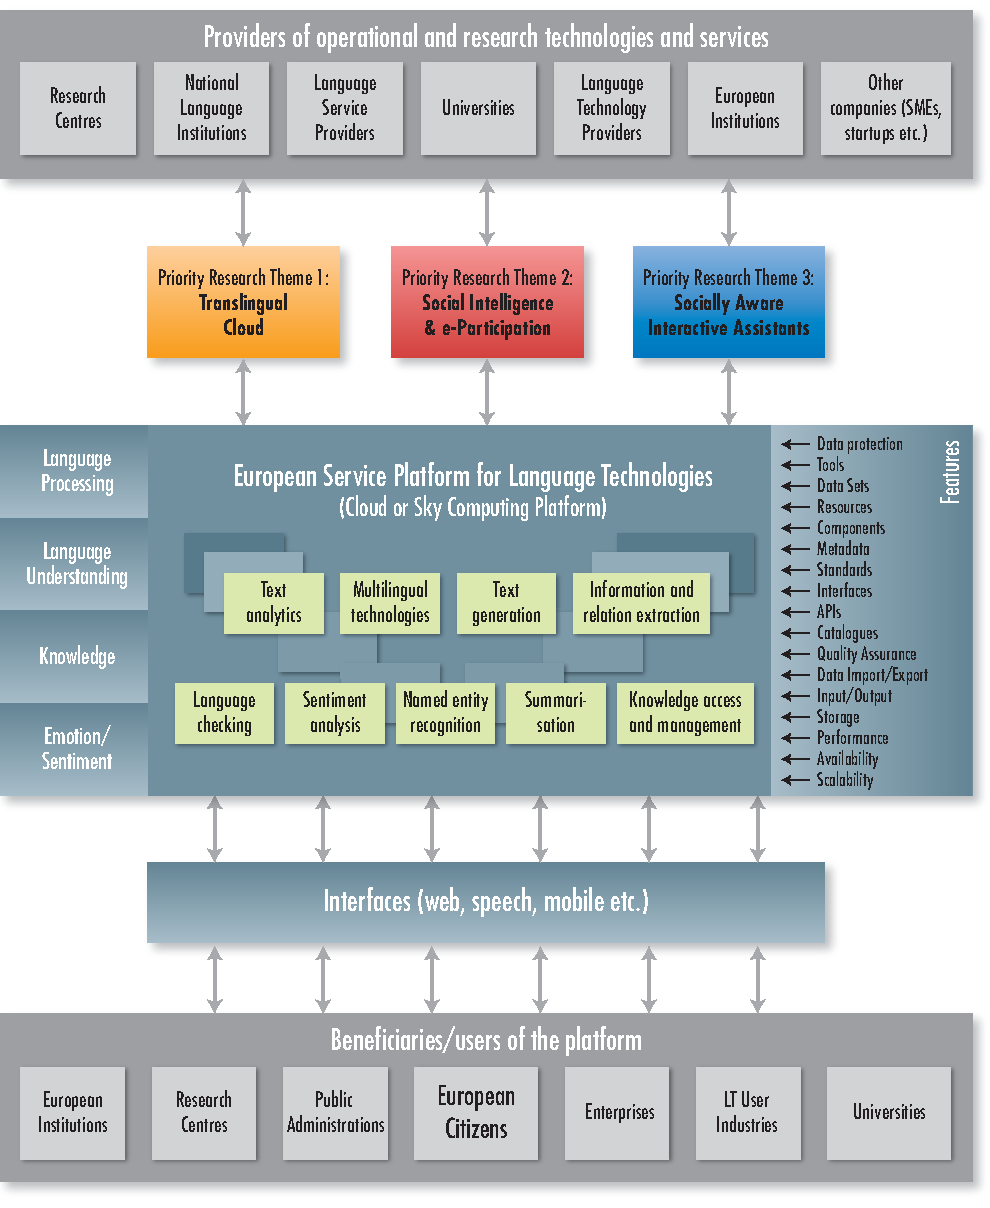
\includegraphics[width=0.83\textwidth]{figures/Platform}
  \caption{European Service Platform for Language Technologies}
  \label{fig:platform-overview}
\end{figure*}

\subsection{Languages to be supported}
\label{sec:languages-to-be-supported}

The \textsc{sra} has a much broader scope in terms of languages to be supported
than our study ``Europe's Languages in the Digital Age''
\citep{LWP2012}. The set of languages to be reflected with
technologies include not only the 23 official languages of the \textsc{eu} but
also recognised and unrecognised regional languages and the languages
of associated countries or non-member states. Equally important are
the minority and immigrant languages that are in active use by a
significant population in Europe (for Germany, these are, among
others, Turkish and Russian; for the \textsc{uk}, these include Bengali,
Urdu/Hindi and Punjabi). An important set of languages outside our
continent are those of important political and trade partners such as Chinese, Japanese, Korean, Russian, and Thai. \textsc{meta-net}
already has good working relationships with several of the respective
official bodies, especially \textsc{efnil} (European Federation of National
Institutions for Language), \textsc{npld} (Network to Promote Linguistic
Diversity), and also the Maaya World Network for Linguistic Diversity.
The concrete composition of languages to be supported by this agenda's
research programme up until the year 2020 and beyond depends on the
composition of participating countries and regions and also on the
specific nature of the funding instruments used and combined for
realising the ambituous plan.

\subsection{Structure and principles of research organisation}
\label{sec:struct-princ-research-org}

The three proposed priority research themes overlap in technologies
and challenges. The overlap reflects the coherence and maturation of
the field. At the same time, the resulting division of labour and
sharing of resources and results is a precondition for the realisation
of this highly ambitious programme. The themes need to benefit from
progress in core technologies of language analysis and production such
as morphological, syntactic and semantic parsing and generation. But
each of the three areas will concentrate on one central area of
language technology: the Translingual Cloud will focus on
cross-lingual technologies such as translation and interpretation; the
Social Intelligence strand will take care of knowledge discovery, text
analytics and related technologies; the research dedicated to
Interactive Assistants will take on technologies such as speech and
multimodal interfaces (see \figref{fig:priority-themes}).

\begin{figure*}[htb]
  \center
  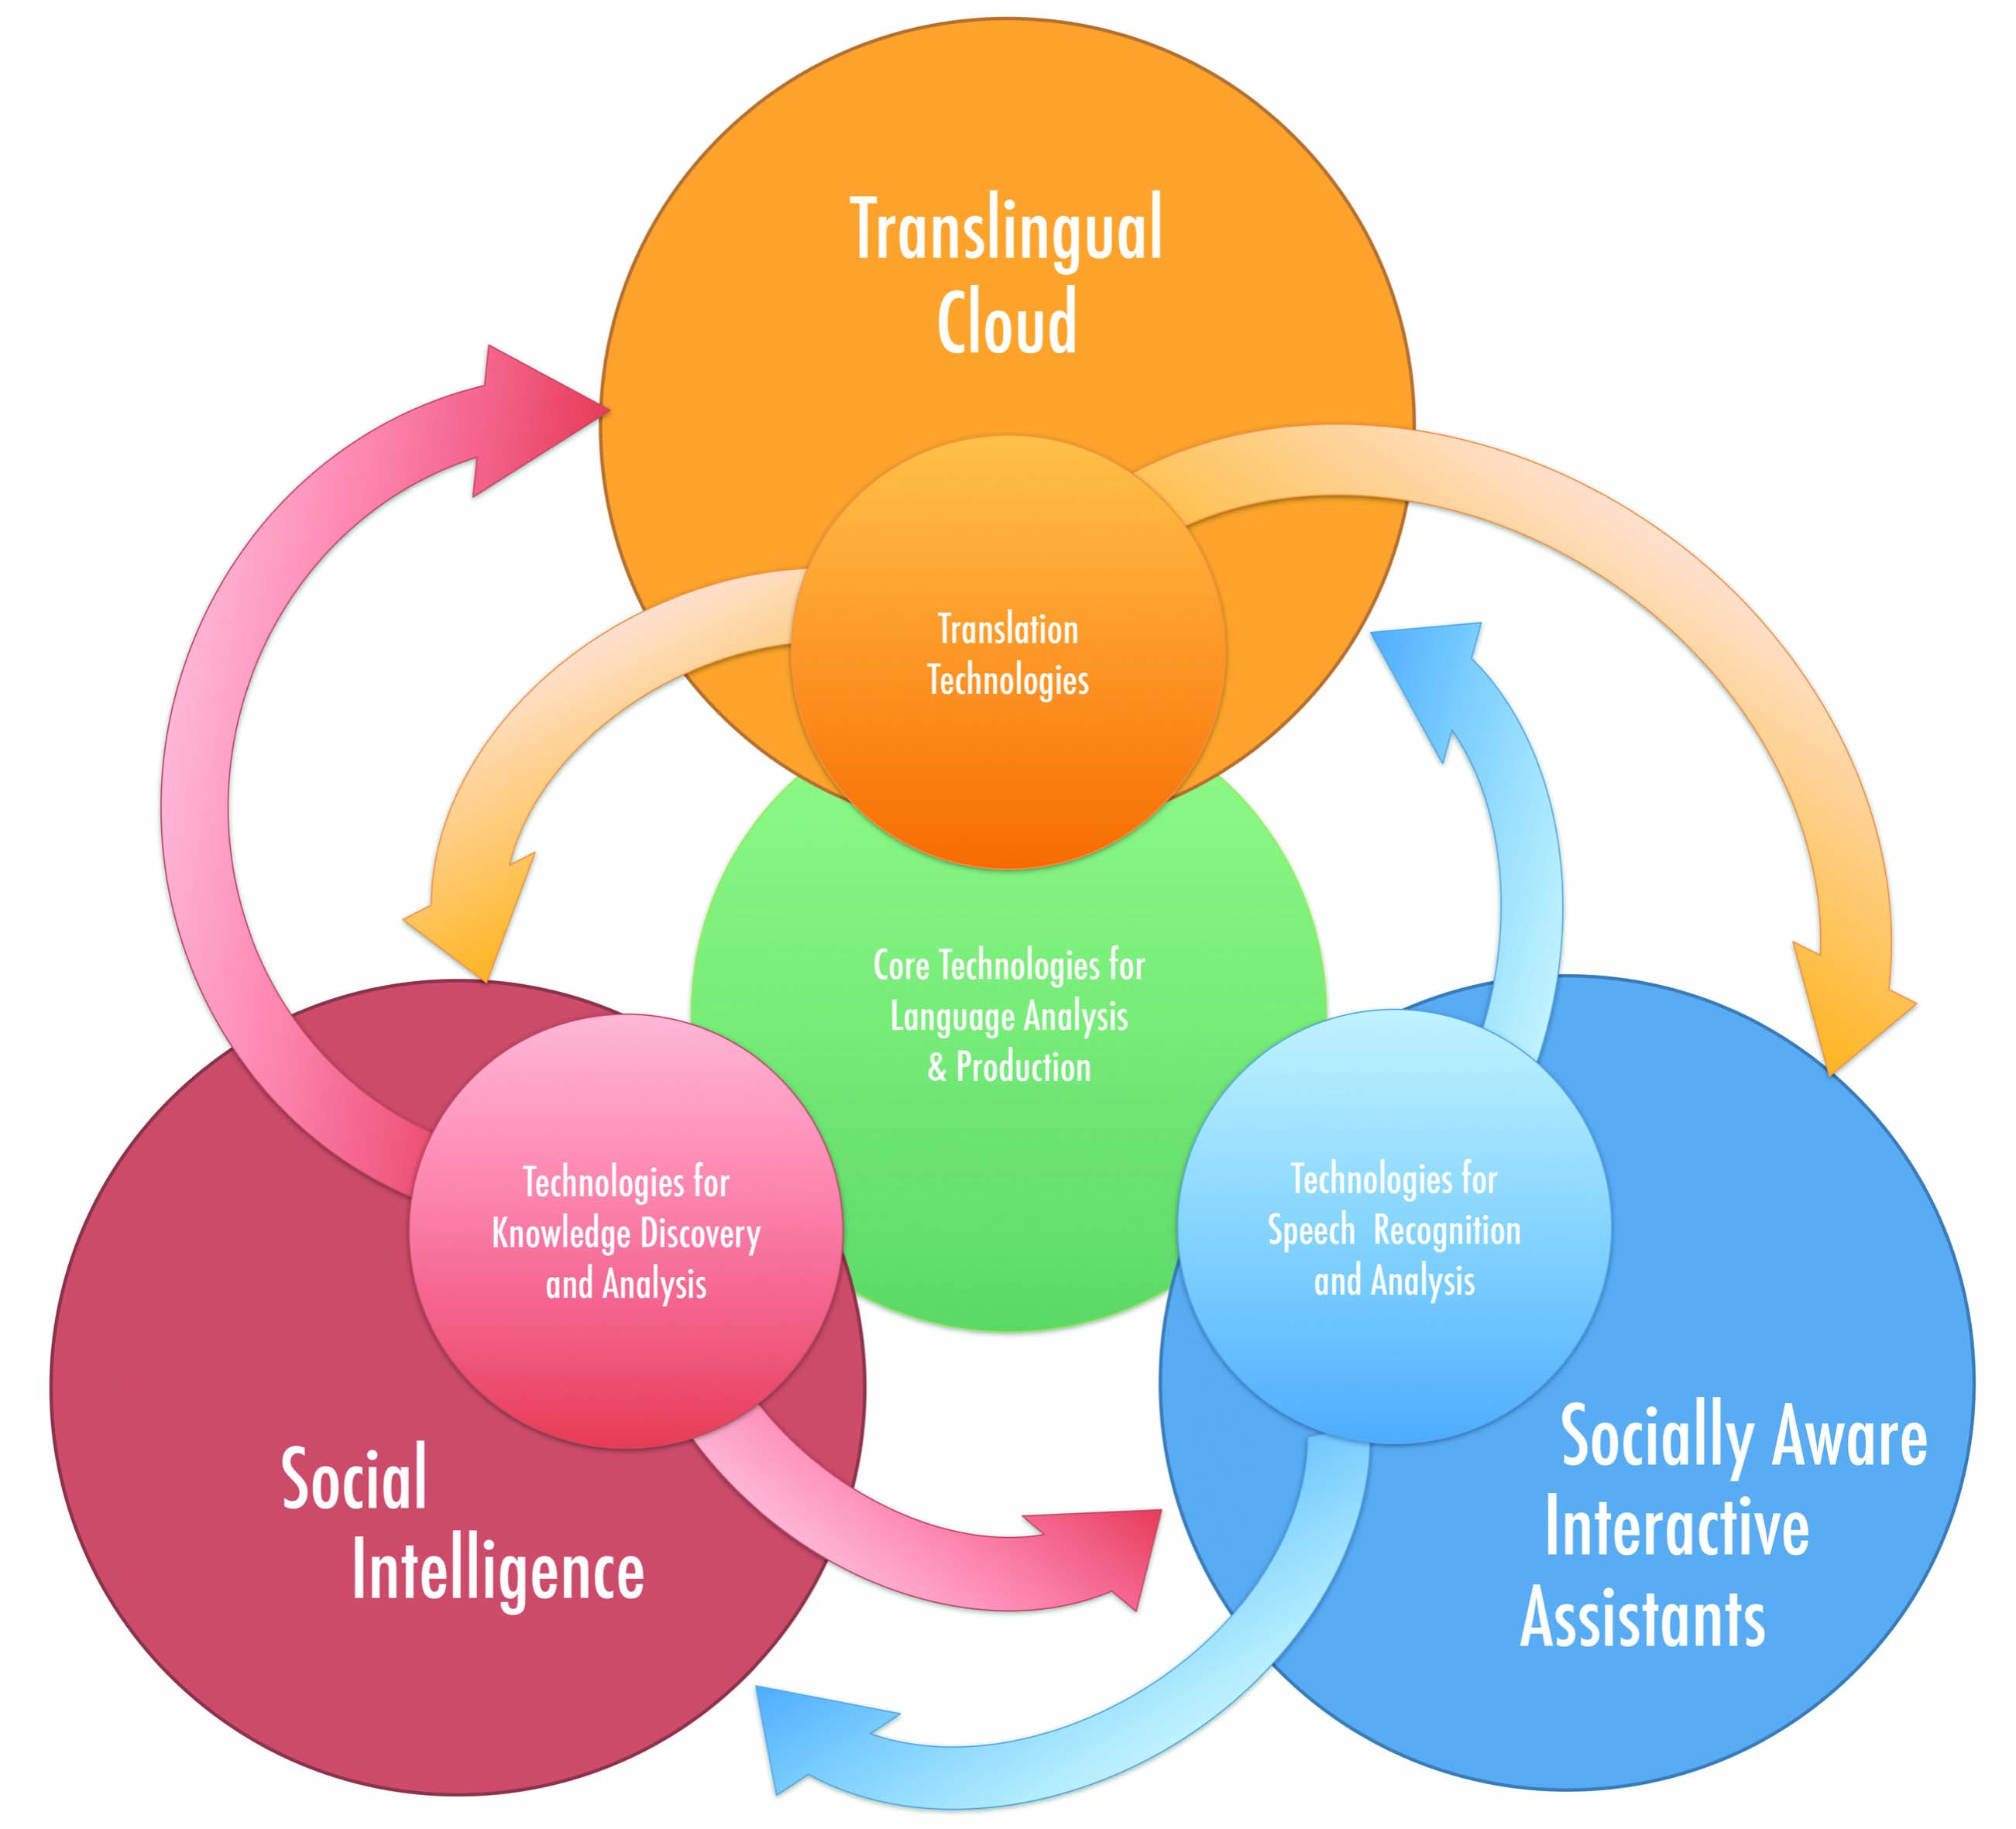
\includegraphics[width=0.5\textwidth]{figures/PT-Rings}
  \caption{Scientific cooperation among the three priority research themes}
  \label{fig:priority-themes}
\end{figure*}

\newpage %Orphan
The final model for the organisation of collaboration will have to be
guided by a thoughtful combination of the following basic
approaches. The collaboration will be interdisciplinary, flexible,
evolutionary and analytical. It will be staged in two major phases
(2015--2017, 2018--2020). We will make heavy use of improving systems
by bootstrapping earlier systems and prototypes and by collaborating
very closely with relevant areas of service and technology industries.

\section{Towards a shared European programme}
\label{sec:summary}

In the Strategic Research Agenda \textsc{meta-net} recommends setting up a
large, multi-year programme on language technologies to build the
technological foundations for a truly multilingual Europe. The
research strands and associated sets of applications we suggest to
build in the next ten years are of utmost importance for
Europe. Through these technologies we will be able to overcome
language barriers in spoken and written communication, we will be able
to carry out country- and language-border-crossing debates and we will
enable new forms and means of communication. We are confident that the
impact of our technologies will be so immense that they will be able
to help establishing a sense of a European identity in the majority of
European citizens. The research plan described in the \textsc{sra} will
generate a countless number of opportunities, it will significantly
participate to Europe's future growth and will secure Europe's
position in many global markets.

Due to the scope and duration of the suggested action, our preferred
option is to set up a shared programme between the European Commission
and the Member States as well as Associated Countries. First steps
along those lines have been taken at \textsc{meta-net}'s \textsc{meta-forum} 2012
conference in Brussels, Belgium, on June 21, 2012, when
representatives of several European funding agencies (Bulgaria, Czech
Republic, France, Hungary, The Netherlands, Slovenia) who participated
in a panel discussion on this topic unanimously expressed the urgent
need for setting up such a shared programme \citep{mf2012}.

The programme will include a carefully planned governance
structure. Here, first steps have been taken as well: \textsc{meta-net} has an
Executive Board with currently 12 members, the operations of the
network and its bodies are specified in its Statutes
\citep{statutes2012}. Furthermore, a legal person for \textsc{meta-net} was
established. This legal person, \textsc{meta-trust} \textsc{aisbl}, is an international
non-profit organisation under Belgian law \citep{metatrust2012}. These
proven and established structures can be used as starting points for
the governance structure of a future programme.

\section*{Acknowledgements}
\label{sec:acknowledgements}

This extended summary of the \emph{\textsc{meta-net} Strategic Research Agenda
  for Multilingual Europe 2020} \citep{SRA2013} is, first and
foremost, based on joint work with the \textsc{sra}'s other co-editor, Hans
Uszkoreit. The work presented in this article would not have been
possible without the dedication and commitment of our colleagues
Aljoscha Burchardt, Kathrin Eichler, Tina Klüwer, Arle Lommel and
Felix Sasaki (all \textsc{dfki}), the 60 member organisations of the \textsc{meta-net}
network of excellence, the ca.~70 members of the Vision Groups, the
ca.~30 members of the \textsc{meta} Technology Council, the more than 200
authors of and contributors to the \textsc{meta-net} Language White Paper
Series \citep{LWP2012} and the ca.~200 representatives from industry
and research who contributed to the \textsc{meta-net} Strategic Research
Agenda. The author would also like to thank the reviewers of this
paper for their helpful comments.

\textsc{meta-net} is co-funded by the 7th Framework Programme of the European
Commission through the following grant agreements: \textsc{t\oldstylenums{4}me} Net
(no.~249\,119), \textsc{cesar} (no.~271\,022), \textsc{metanet\oldstylenums{4}u} (no.~270\,893) and
\textsc{meta-nord} (no.~270\,899).

More information is available at \url{http://www.meta-net.eu} and via
\url{office@meta-net.eu}.

 


\sloppy
\printbibliography[heading=subbibliography,notkeyword=this]

\end{document}
